\documentclass[Arkitektur/System_main.tex]{subfiles}
\begin{document}
\subsubsection{Tilføjelse og fjernelse af bil profil}
I dette afsnit beskrives funktionaliteten, når en bruger ønsker at tilføje sin bil til udlejning ved at lave en bilprofil, samt når en bruger ønsker at slette bil profillen igen.
\textbf{Tilføje bil profil}
Til at beskrive arkitekturen for at tilføje en bil er der lavet et sekvensdiagram, der viser samspillet mellem bruger applikation og database. Dette diagram kan ses nedenfor i figur \ref{fig:RegisterCarProfileSD}.
\begin{figure}[H]
    \centering
    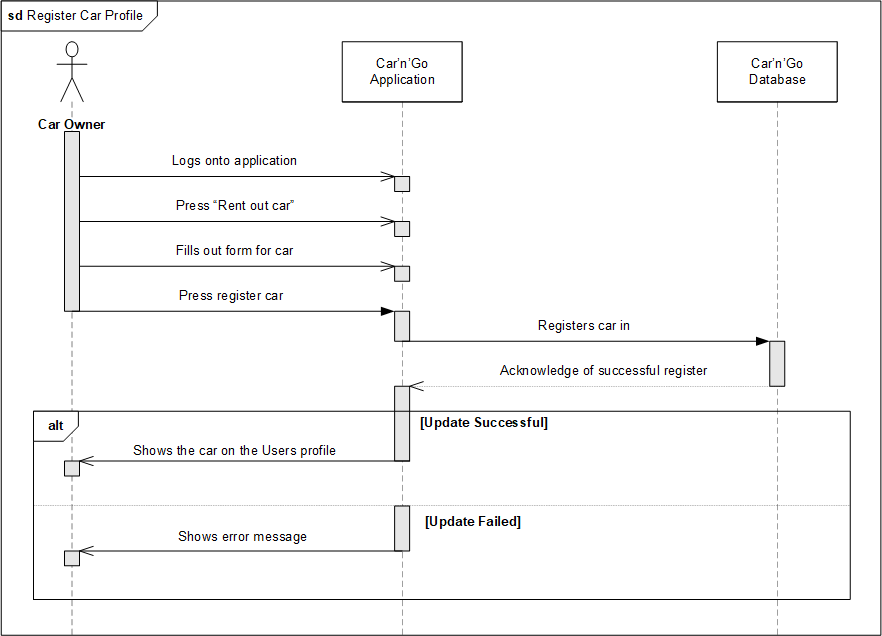
\includegraphics[width=1\textwidth]{Arkitektur/Softwarearkitektur/Car_registration/graphics/RegisterCarSD.png}
    \caption{Her ses et sekvensdiagram for samspillet mellem udlejer, applikation og database. }
    \label{fig:RegisterCarProfileSD}
\end{figure}
Der er også lavet en applikationsmodel, som består af et klassediagram, som ses på figur \ref{fig:RegisterCarProfileCD}, og et statemachine diagram, som ses på figur \ref{fig:RegisterCarProfileSTM}.
\begin{figure}[H]
    \centering
    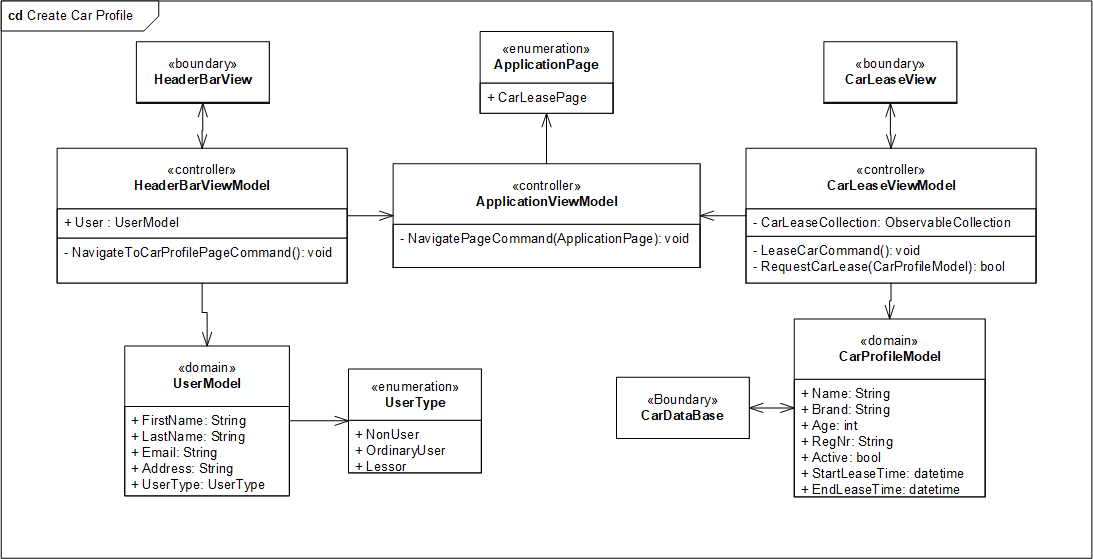
\includegraphics[width=1\textwidth]{Arkitektur/Softwarearkitektur/Car_registration/graphics/RegisterCarProfileCD.png}
    \caption{Her ses klassediagrammet for tilføjelse af bil til en brugerprofil. }
    \label{fig:RegisterCarProfileCD}
\end{figure}

\begin{figure}[H]
    \centering
    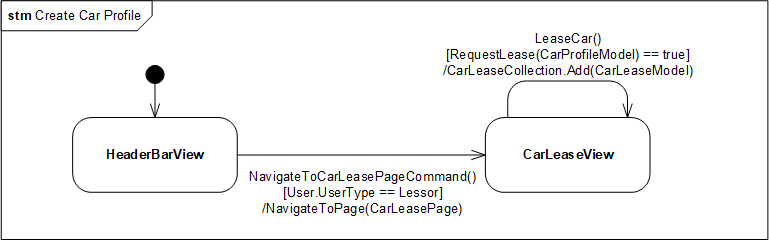
\includegraphics[width=1\textwidth]{Arkitektur/Softwarearkitektur/Car_registration/graphics/RegisterCarProfileSTM.png}
    \caption{Her ses Statemachinediagram for tilføjelse af bil til en brugerprofil. }
    \label{fig:RegisterCarProfileSTM}
\end{figure}
\textbf{Fjernelse af bil profil}
Når en bruger ikke længere ønsker at udleje sin bil, så skal brugeren slette bilprofilen. Arkitekturen for denne funktionalitet er beskrevet med et sekvensdiagram for samspillet mellem udlejer, applikation og database, samt en applikationmodel. Sekvensdiagrammet ses nedenfor på figur \ref{fig:DeleteCarProfileCD}

\begin{figure}[H]
    \centering
    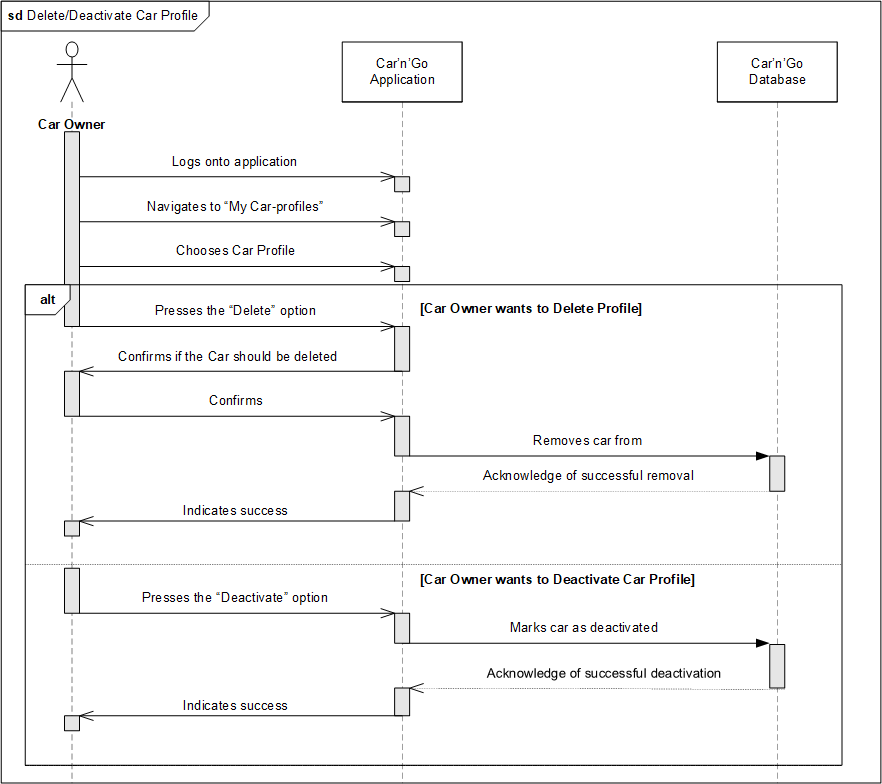
\includegraphics[width=1\textwidth]{Arkitektur/Softwarearkitektur/Car_registration/graphics/DeleteCarProfileSD.png}
    \caption{Her ses sekvensdiagrammet for fjernelsen af en bilprofil, som viser samspillet mellem udlejer, applikation og database. }
    \label{fig:DeleteCarProfileCD}
\end{figure}



Applikationsmodellen består af et klassediagram, samt en satemachine, hvor klassediagrammet ses på figur \ref{fig:RemoveDeactivateCarProfileCD} og et statemachine diagram, som ses på figur \ref{fig:RemoveDeactivateCarProfileSTM}.
\begin{figure}[H]
    \centering
    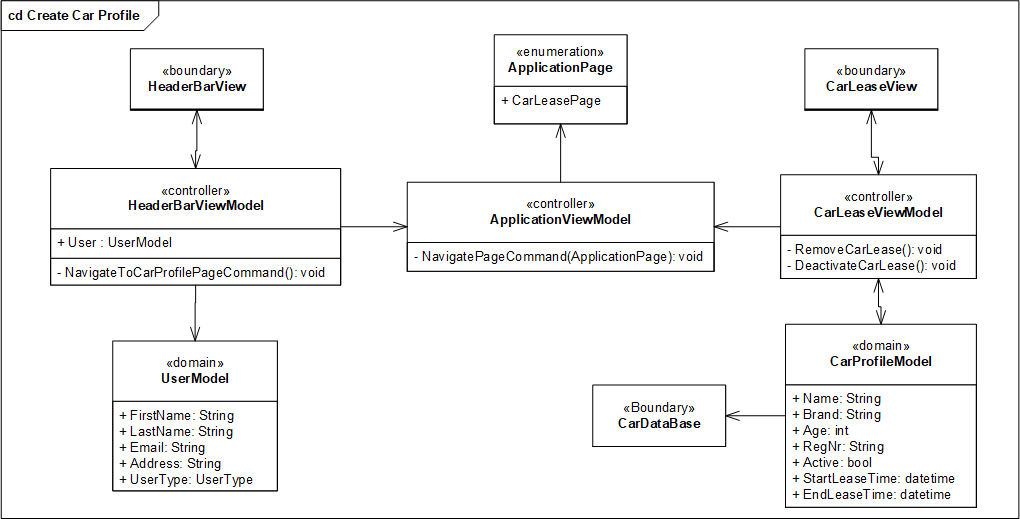
\includegraphics[width=1\textwidth]{Arkitektur/Softwarearkitektur/Car_registration/graphics/RemoveDeactivateCarProfileCD.png}
    \caption{Her ses klassediagrammet for fjernelse af bil fra en brugerprofil. }
    \label{fig:RemoveDeactivateCarProfileCD}
\end{figure}

\begin{figure}[H]
    \centering
    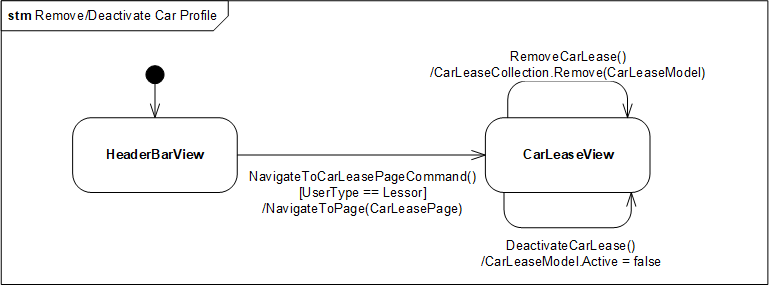
\includegraphics[width=1\textwidth]{Arkitektur/Softwarearkitektur/Car_registration/graphics/RemoveDeactivateCarProfileSTM.png}
    \caption{Her ses statemachine for fjernelse af bil fra en brugerprofil. }
    \label{fig:RemoveDeactivateCarProfileSTM}
\end{figure}





\end{document}